%%%%%%%%%%%%%%%%%%%%%%%%%%%%%%%%%%%%%%%%%%%%%%%%%%%%%%%%%%%%%%%%%%%%%%%%%%%%%%%%
%%%%%%%%%%%%%%%%%%%%%%%%%%%%%%%%%%%%%%%%%%%%%%%%%%%%%%%%%%%%%%%%%%%%%%%%%%%%%%%%
%%% Template for AIMS Rwanda Assignments         %%%              %%%
%%% Author:   AIMS Rwanda tutors                             %%%   ###        %%%
%%% Email: tutors2017-18@aims.ac.rw                               %%%   ###        %%%
%%% Copyright: This template was designed to be used for    %%% #######      %%%
%%% the assignments at AIMS Rwanda during the academic year %%%   ###        %%%
%%% 2017-2018.                                              %%%   #########  %%%
%%% You are free to alter any part of this document for     %%%   ###   ###  %%%
%%% yourself and for distribution.                          %%%   ###   ###  %%%
%%%                                                         %%%              %%%
%%%%%%%%%%%%%%%%%%%%%%%%%%%%%%%%%%%%%%%%%%%%%%%%%%%%%%%%%%%%%%%%%%%%%%%%%%%%%%%%
%%%%%%%%%%%%%%%%%%%%%%%%%%%%%%%%%%%%%%%%%%%%%%%%%%%%%%%%%%%%%%%%%%%%%%%%%%%%%%%%


%%%%%% Ensure that you do not write the questions before each of the solutions because it is not necessary. %%%%%% 

\documentclass[12pt,a4paper]{article}

%%%%%%%%%%%%%%%%%%%%%%%%% packages %%%%%%%%%%%%%%%%%%%%%%%%
\usepackage{amsmath}
\usepackage{amssymb}
\usepackage{amsthm}
\usepackage{amsfonts}
\usepackage{graphicx}
\usepackage[all]{xy}
\usepackage{tikz}
\usepackage{verbatim}
\usepackage[left=2cm,right=2cm,top=3cm,bottom=2.5cm]{geometry}
\usepackage{hyperref}
\usepackage{caption}
\usepackage{subcaption}
\usepackage{psfrag}

%%%%%%%%%%%%%%%%%%%%% students data %%%%%%%%%%%%%%%%%%%%%%%%
\newcommand{\student}{Akor Stanley}
\newcommand{\course}{PDE2\left(  }
\newcommand{\assignment}{1}

%%%%%%%%%%%%%%%%%%% using theorem style %%%%%%%%%%%%%%%%%%%%
\newtheorem{thm}{Theorem}
\newtheorem{lem}[thm]{Lemma}
\newtheorem{defn}[thm]{Definition}
\newtheorem{exa}[thm]{Example}
\newtheorem{rem}[thm]{Remark}
\newtheorem{coro}[thm]{Corollary}
\newtheorem{quest}{Question}[section]

%%%%%%%%%%%%%%  Shortcut for usual set of numbers  %%%%%%%%%%%

\newcommand{\N}{\mathbb{N}}
\newcommand{\Z}{\mathbb{Z}}
\newcommand{\Q}{\mathbb{Q}}
\newcommand{\R}{\mathbb{R}}
\newcommand{\C}{\mathbb{C}}
%%%%%%%%%%%%%%%%%%%%%%%%%%%%%%%%%%%%%%%%%%%%%%%%%%%%%%%555
\begin{document}
%%%%%%%%%%%%%%%%%%%%%%% title page %%%%%%%%%%%%%%%%%%%%%%%%%%
\thispagestyle{empty}
\begin{center}
\textbf{AFRICAN INSTITUTE FOR MATHEMATICAL SCIENCES \\[0.5cm]
(AIMS RWANDA, KIGALI)}
\vspace{1.0cm}
\end{center}
%%%%%%%%%%%%%%%%%%%%% assignment information %%%%%%%%%%%%%%%%
\noindent
\rule{17cm}{0.2cm}\\[0.3cm]
Name: \student \hfill Assignment Number: \assignment\\[0.1cm]
Course: \course \hfill Date: \today\\
\rule{17cm}{0.05cm}
\vspace{1.0cm}
\section*{Question 1}
\begin{itemize}
	\item [(a)] The fourier series for $f(x)=e^{ax}$ is given by;
	\begin{align}
	f(x)=\frac{a_{\circ}}{2}+\sum_{n=1}^{\infty} (a_{n}\cos (n\pi x)+b_{n}\sin (n\pi x)) \label{1}
	\end{align}
	Let us determine the coeffiecients ${a_{\circ}, b_{n}, a_{n}}$ of $f(x)$.
	\begin{align*}
	a_{\circ}&=\frac{1}{\pi}\int_{-\pi}^{\pi} e^{ax} dx\\
	&=\frac{1}{\pi}\left[\frac{e^{ax}}{a}\right]^{\pi}_{-\pi }\\
	&=\frac{1}{\pi}\left[ \frac{e^{\pi a}}{a}-\frac{e^{-\pi a}}{a}\right]\\
	&=\frac{1}{\pi a}(e^{\pi a}-e^{-\pi a})
	\end{align*}
	But, $\sinh \pi a=\frac{1}{2}\left(e^{\pi a}-e^{-\pi a}\right)$, so that $a_{\circ}$ becomes;
	\begin{align*}
	a_{\circ}=\frac{2}{\pi a} \sinh (\pi a)
	\end{align*}
	\begin{align}
	a_{n}&=\frac{1}{\pi}\int_{-\pi}^{\pi}f(x)\cos(n x)\\
	&=\frac{1}{\pi}\int_{-\pi}^{\pi}e^{ax}\cos(n x)dx
	\end{align}
	But the trigonometic function has its complex representation as; $\cos(n\pi x)=\frac{1}{2}\left(e^{in\pi x}+e^{-in\pi x}\right)$ 
	\begin{align*}
	a_{n}&=\frac{1}{2\pi}\int_{-\pi}^{\pi}e^{ax}\left(e^{i n x}+e^{-in x}\right)dx\\
	&=\frac{1}{2\pi}\int_{-\pi}^{\pi}e^{(a+in )x}+e^{(a-in)x}dx\\
	&=\frac{1}{2\pi}\left(\left[\frac{e^{(a+in)x}}{a+in}+\frac{e^{(a-in\pi )x}}{a-in}\right]^{\pi}_{-\pi}\right)\\
	&=\frac{1}{2\pi}\left[\frac{(a-in)e^{x(a+in)}+(a-in)e^{x(a-in)}}{a^{2}+n^{2}}\right]^{\pi}_{-\pi}\\
	&=\frac{1}{2\pi(a^{2}+b^{2})}\left[2ae^{ax}\cos(nx)+2ie^{ax}\sin(nx)\right]^{\pi}_{-\pi}
	\end{align*}
	Since $\cos(n\pi)=(-1)^{n}$,  $\cos(-n\pi)=(-1)^{n}$, and $\cos(0)=1$. We will then have;
	\begin{align*}
	a_{n}&=\frac{1}{\pi}\left(\frac{a(-1)^{n}(e^{a\pi}-e^{-a\pi})}{(a^{2}+n^{2})}\right)\\
	&=\frac{2}{\pi}\left(\frac{a(-1)^{n}\sinh (a\pi)}{(a^{2}+n^{2})}\right)
	\end{align*}
	The third fourier coeficient  $b_{n}$ is obtained as follows;
	\begin{align*}
	b_{n}=&=\frac{1}{\pi}\int_{-\pi}^{\pi}f(x)\sin(n x)dx\\
	&=\frac{1}{\pi}\int_{-\pi}^{\pi}e^{ax}\sin(n x)dx\\
	&=\frac{1}{2i\pi}\int_{-\pi}^{\pi}e^{ax}\left(e^{i n x}-e^{-in x}\right)dx\\
	&=\frac{1}{2i\pi}\int_{-\pi}^{\pi}e^{(a+in )x}-e^{(a-in)x}dx\\
	&=\frac{1}{2\pi}\left[-i\frac{ (a-in)e^{x(a+in)}-(a-in)e^{x(a-in)}}{a^{2}+n^{2}}\right]^{\pi}_{-\pi}\\
	&=\frac{1}{2\pi}\left[-i\frac{2ne^{ax}\cos(nx)-2ae^{ax}\sin(nx)}{\left(a^{2}+n^{2}\right)}\right]^{\pi}_{-\pi}\\
	&=\frac{2}{\pi}\left(\frac{n(-1)^{n+1}\sinh (a\pi)}{(a^{2}+n^{2})}\right)
	\end{align*}
	Now substituting $a_{n},b_{n}, a_{\circ}$ into equation(\ref{1}), we shall obtain;
	\begin{align}
	e^{ax}&=\frac{1}{\pi a} \sinh (\pi a)+\sum_{n=1}^{\infty}\left(\frac{2}{\pi}\left(\frac{a(-1)^{n}\sinh (a\pi)}{(a^{2}+n^{2})}\right)\cos(nx)+\frac{2}{\pi}\left(\frac{n(-1)^{n+1}\sinh (a\pi)}{(a^{2}+n^{2})}\right)\sin(nx)\right)\\
	&=\frac{1}{\pi a} \sinh (\pi a)+2\sum_{n=1}^{\infty}\left(\frac{(-1)^{n}}{\pi (a^{2}+n^{2})}(a\cos(nx)-n\sin(nx))\right)\sinh(a\pi) \label{2}
	\end{align}
	\item [(b)] We want to evalute $g(x)=\sinh x$, using equation(\ref{2}). It follows that;
	\begin{align*}
	g(x)&=\frac{1}{2}\left(e^{x}-e^{-x}\right)\\
	&=\frac{1}{2}\left([e^{ax}]_{a=1}-[e^{ax}]_{a=-1}\right)\\
	\end{align*}
	It follows that by substiuting $a=-1$ in equaion(\ref{2}), and performing the expansion, even terms will cancel out living us with this simplified fucntion;
	\begin{align*}
	g(x)=\frac{\sinh (\pi )}{\pi }\left(2\sum_{n=1}^{\infty}\left(\frac{(-1)^{n+1}\sinh (\pi)}{(1+n^{2})}\right)-n\sin(nx)\right)
	\end{align*}
\end{itemize}
\section*{Question 2}
\begin{itemize}
\item[(a)]
\begin{align*}
\frac{1}{c^{2}}\frac{\partial ^{2}U}{\partial t^{2}}=\frac{\partial ^{2}U}{\partial x^{2}}
\end{align*}
We start of by guessing that $U(x,t)=X(x)T(t)$ is a solution to the above equation.
\begin{align*}
\frac{\partial U}{\partial x}=X^{\prime}T \quad \frac{\partial^{2} U}{\partial x^{2}}={X^{\prime}}^{\prime}T\\
\frac{\partial U}{\partial t}=\dot{T}X \quad \frac{\partial^{2} U}{\partial t^{2}}=\ddot{T}X
\end{align*}
Substituting these into the original equation, we obtain;
\begin{align}
\frac{1}{c^{2}}\ddot{T}X={X^{\prime}}^{\prime}T \label{3}
\end{align}
Dividing equation(\ref{3}) by $X(x)T(t)$, we shall obtain;
\begin{align}
\frac{\ddot{T}}{c^{2}T}&=\frac{{X^{\prime}}^{\prime}}{X}=\lambda\\
\ddot{T}-c^{2}T\lambda &=0 \label{5}\\
{X^{\prime}}^{\prime}-X\lambda&=0 \label{4}
\end{align}
Let us solve the linear equation(\ref{4}), we shall consider three cases.\\
\textbf{Case 1} $\lambda >0$, so let $\lambda=\mu^{2}$ with $\mu \neq 0$. Equation(\ref{4}) now becomes;
\begin{align}
{X^{\prime}}^{\prime}-X\mu^{2}&=0 \label{6}
\end{align}
The solution  to equation(\ref{6}) is $X(x)=Ae^{\mu x}+Be^{-\mu x}$. By applying the boundary condition on X gives only the trivial solution, where $A=0$, and $B=0$.\\
\newline
\textbf{Case 2} $\lambda =0$. Equation(\ref{4}) now becomes;
\begin{align}
{X^{\prime}}^{\prime}&=0 \label{7}
\end{align}
The solution to equation(\ref{7}), is given by;
\begin{align}
X(x)=Ax+B \label{8}
\end{align}
By applying the boundary conditions on equation(\ref{8}), we obtain;
\begin{align*}
X_{\circ}(x)=A_{\circ}
\end{align*}
\textbf{Case 3} $\lambda <0$, so let $\lambda=-\mu^{2}$ with $\mu \neq 0$. Equation(\ref{4}) now becomes;
\begin{align}
{X^{\prime}}^{\prime}+X\mu^{2}&=0 \label{9}
\end{align}
The solution to equation(\ref{9}) is given by;
\begin{align*}
X(x)=A\cos(\mu x)+B\sin(\mu x)
\end{align*}
Applying the boundary conditions;
\begin{align*}
X^{\prime}&=B\mu \cos(\mu x)-A\mu \sin(\mu x)=0\\
X^{\prime}(0)&=B=0
\end{align*}
The solution for $X(x)$ now becomes;
\begin{align*}
X(x)=A \cos(\mu x)
\end{align*}
\begin{align*}
X^{\prime}(1)&=-A\mu \sin(\mu )=0\\ 
&A\mu \sin(\mu )=0
\end{align*}
Since $\mu \neq 0$, it therefore means that $\sin(\mu)=0$. The corresponding values of $\mu$ for which $\sin(\mu)=0$ are;
\begin{align*}
\mu&=n\pi 			\quad \quad \quad n\in \Z\\ 		
\therefore \lambda_{n}&=-(n\pi)^{2}
\end{align*}
Where $\lambda_{n} $ is defined as the eigen value. Now from equation(\ref{5})
\begin{align}
\ddot{T}-c^{2}T\lambda&=0\\
\ddot{T}+(cn\pi)^{2}T&=0\label{8}
\end{align}
The solution of equation(\ref{8}) is given by;
\begin{align}
T_{n}(t)=C_{n}\cos(n\pi ct)+D_{n}\sin (n\pi ct) \label{10}
\end{align}
By applying the initial condition of $\dot{T}(0)=0$, it follows that $D_{n}$ varnishes, leaving us with;
$$T_{n}(t)=C_{n}\cos(n\pi ct)$$
The final solution $U(x,t)$ is obtained by combining the solutions of $T$ and $X$ as shown below;
\begin{align*}
U_{n}=A_{n}\cos(n\pi x)\cos(n\pi ct)
\end{align*}
We use the fact that the wave equation is linear to superpose the solutions which yields the general solution.
\begin{align}
U(x,t)=A_{\circ}+\sum_{n=1}^{\infty}A_{n}\cos(n\pi ct)\cos(n\pi x) \label{11}
\end{align}
\item [(b)]
By Applying equation(\ref{11}), we set $g(x)=U(x,0)$. So that $\cos(n\pi ct)=1$;
\begin{align}
g(x)=A_{\circ}+\sum_{n=1}^{\infty}A_{n} \cos(n\pi x) \label{12}
\end{align}
Equation(\ref{12}) is a fourier series, with $A_{\circ}=\frac{a_{0}}{2}$, $A_{n}=a_{n}$ and $b_{n}=0$. Because the obtained function is even, we can apply the half range formular;
\begin{align*}
a_{\circ}&=2\int^{\frac{1}{2}}_{0}g(x)dx\\
&=2\int^{\frac{1}{2}}_{0}1 dx\\
&=1
\end{align*}
Similary;
\begin{align*}
a_{n}&=2\int^{\frac{1}{2}}_{0} g(x)\cos(n\pi x)dx\\
&=2\int^{\frac{1}{2}}_{0}\cos(n\pi x)dx\\
&=\frac{2}{n\pi}\left[\sin(n\pi x)\right]^{\frac{1}{2}}_{0}\\
&=\frac{2}{n\pi}\sin(\frac{n\pi}{2})
\end{align*}
The general solution now becomes;
\begin{align}
U(x,t)=\frac{1}{2}+\sum_{n=1}^{\infty}\frac{2}{n\pi}\sin(\frac{n\pi}{2})\cos(n\pi ct)\cos(n\pi x) \label{13} 
\end{align}
It follows that for even $n$, the summation is zero, because $\sin(\frac{n\pi}{2})$ will be zero. For odd $n$, we set $n=2k-1$, so that equation(\ref{13}) becomes;
\begin{align*}
U(x,t)=\frac{1}{2}+\sum_{k=1}^{\infty}\frac{2(-1)^{k+1}}{\pi(2k-1)}\cos((2k-1)\pi ct)\cos((2k-1)\pi x)
\end{align*}
\end{itemize}
\newpage
\section*{Question 3}
\begin{itemize}
	\item [(a)]
	.\\
	\begin{figure}[h!]
		\centering
		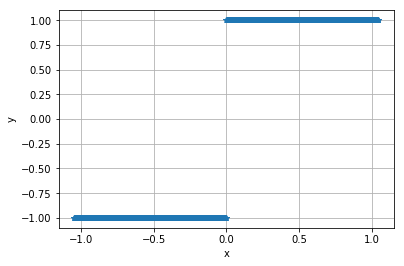
\includegraphics[scale=0.6]{Image1.png}
		\caption{Odd extension of f(x)}
	\end{figure}
	
	Since the function is odd, we can conveniently apply the half range formular. $a_{0}=a_{n}=0$
	\begin{align*}
	b_{n}&=\frac{2}{\pi}\int_{0}^{\pi}\sin(m x)dx\\
	&=\frac{2}{\pi}\left[\frac{-\cos(m  x)}{n}\right]^{\pi}_{0}\\
	&=\frac{2}{m\pi}\left(1-(-1)^{m}\right)
	\end{align*}
	For even $m$, $b_{m}$ becomes zero, but for odd $m$ we set, $m=2n-1$, we have $b_{m}=\frac{4}{m\pi}$;
	\begin{align}
	f(x)&=\sum_{n=1}^{\infty}\frac{4}{(2n-1)\pi}\sin((2n-1) x)\\
	&=\frac{4}{\pi}\sum_{n=1}^{\infty}\frac{\sin((2n-1) x)}{2n-1} \label{15}
	\end{align}
	\newpage
	\item[(b)]
	.\\
	\begin{figure}[h!]
		\centering
		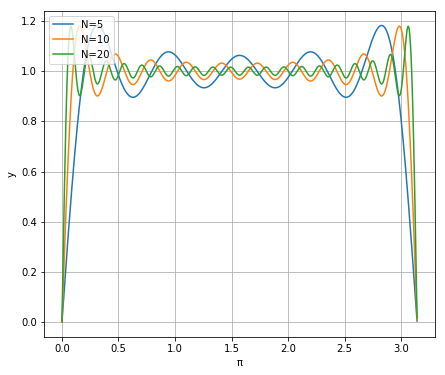
\includegraphics[scale=0.6]{Image2.png}
		\caption{The partial sum of the fourier series}
	\end{figure}

	\begin{figure}[h!]
		\centering
		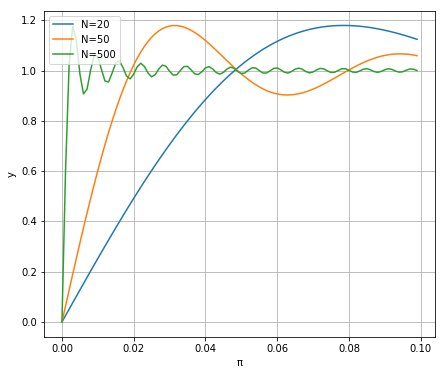
\includegraphics[scale=0.6]{Image3.png}
		\caption{The partial sum of the fourier series} \label{22}
	\end{figure}
	\newpage
	\item [(c)] 
	From equation(\ref{15}), we have;
	\begin{align*}
	F_{N}(x)&=\frac{4}{\pi}\sum_{n=1}^{N}\frac{\sin((2n-1) x)}{2n-1}\\
	F_{N}^{\prime}&=\frac{4}{\pi}\sum_{n=1}^{N}\cos((2n-1)x)
	\end{align*}
	Multiplying both sides by $\sin x$, we shall obtain;
	\begin{align}
	\sin(x)F_{N}^{\prime}=\frac{4}{\pi}\sum_{n=1}^{N}\cos((2n-1)x)\sin(x) \label{19}
	\end{align}
	Given; 
	\begin{align}
	\sum_{n=1}^{N}\sin(x)\cos((2n-1)x)=\frac{1}{2}\sin(2Nx) \label{20}
	\end{align}
	Equation(\ref{19}) 
	\begin{align*}
	\sin(x)F_{N}^{\prime}&=\frac{2}{\pi}\sin(2Nx)\\
	F_{N}^{\prime}&=\frac{\sin(2Nx)}{\sin(x)}\\
	F_{N}&=\int_{0}^{x}\frac{\sin(2Nt)}{\sin(t)} dt
	\end{align*}
	Hence Shown!!!\\
	\newline
	To prove the relation given in the hint, equation(\ref{20}); We apply the double angle relations $i.e$
	\begin{align*}
	\sin(a+b)&=\sin(a)\cos(b)+\sin(b)\cos(a)\\
	\sin(a-b)&=\sin(a)\cos(b)-\sin(b)\cos(a)\\
	\therefore&\\
	\sin(a)\cos(b)&=\frac{1}{2}\left(\sin(b+a)-\sin(b-a)\right)
	\end{align*}
	Applying the double angle relations on the given problem, we shall obtain;
	\begin{align*}
	\sin(x)\cos((2n-1)x)=\frac{1}{2}\left(\sin(2nx)-\sin(2(n-1)x)\right)
	\end{align*}
	Which then leads to;
	\begin{align*}
	\sum_{n=1}^{N}\sin(x)\cos((2n-1)x)&=\frac{1}{2}\sum_{n=1}^{N}\left(\sin(2nx)-\sin(2(n-1)x)\right)\\
	&=\sin(2Nx)-\sin((2N-1)x)+\sin(2(N-1)x)-\sin(2(N-2)x)\\
	&+\sin(2(N-2)x)+\sin(2(N-3)x)-\sin(2(N-3)x)+...+\\
	&+\sin(2x)-\sin(2x)+\sin(x)-\sin(x)-sin(0)\\
	&=\frac{1}{2}\left(\sin(2Nx)\right) 
	\end{align*}
	Notice that alomost all the terms cancel out in the summation, leaving us with just $\sin(2Nx)$
	
	\item [(d)]
	The actual value of the integral obtained from python is $1.1789797444721675$. Notice that this result is comparable to what we obtained in our previous plots(\ref{22}) when we consider the peak values of the curves. The computational results indicates that the maximum error in the fourier approximation does not disappear as $N$ continues to increase, but the extremas tend to the point of discontinuity, and therefore the function cannot be defined within this region.\\
	\newline
	The covergence principle holds as convergence acts on a fixed point $x$ to some value $N$ as it tends to infinity, the limit will converge everywhere except for the point of discontinuity. Because $x=\frac{\pi}{2N}$ is fixed, we conclude that the fourier convergence theorem holds.
	
\end{itemize}
	
\end{document}